\documentclass{standalone}
\usepackage{tikz}
\usetikzlibrary{calc}
\begin{document}
	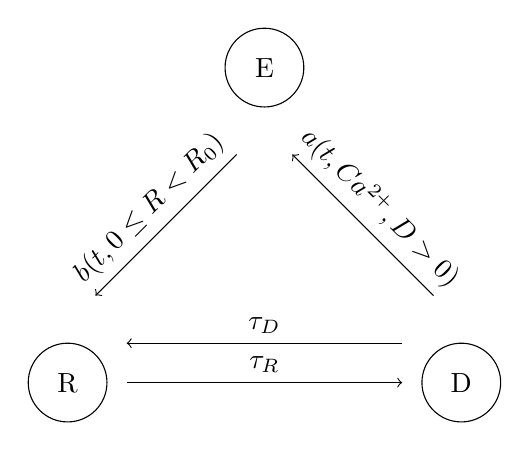
\begin{tikzpicture}
		% Adjustments for a wider triangle base
		\def\triangleBase{5}
		\def\triangleHeight{4}
		
		% Position of R, D, and E circles
		\coordinate (R) at (0,0);
		\coordinate (D) at (\triangleBase,0);
		\coordinate (E) at (\triangleBase/2,\triangleHeight);
		
		% Draw the circle with label "R"
		\draw (R) circle (0.5);
		\node at (R) {R};
		
		% Draw the circle with label "D"
		\draw (D) circle (0.5);
		\node at (D) {D};
		
		% Draw the circle with label "E"
		\draw (E) circle (0.5);
		\node at (E) {E};
		
		% Draw the arrow going from "R" to "D" with "b" on top
		\draw[->] ([xshift=0.75cm]R) -- ([xshift=-0.75cm]D);
		\node[above] at ($ (R)!0.5!(D) $) {$\tau_R$};
		
		% Draw the arrow returning from "D" to "R" with "a" on top
		\draw[->] ([xshift=-0.75cm,yshift=0.5cm]D) -- ([xshift=0.75cm,yshift=0.5cm]R);
		\node[above] at ($ (R)!0.5!(D) + (0,0.5) $) {$\tau_D$};
		
		% Draw an arrow going from "R" to "E" (reacidification)
		\draw[<-, shorten >=0.5cm, shorten <=0.5cm] ([yshift=0.75cm]R) -- ([yshift=-0.75cm]E) node[midway,sloped,above] {${b(t, 0 \le R<R_0)}$};
		
		% Draw an arrow going from "D" to "E" (alkalinization)
		\draw[->, shorten >=0.5cm, shorten <=0.5cm] ([yshift=0.75cm]D) -- ([yshift=-0.75cm]E) node[midway,sloped,above] {${a(t,Ca^{2+}, D>0)}$};
	\end{tikzpicture}
\end{document}


%\documentclass{standalone}
%\usepackage{tikz}
%\begin{document}
%	\begin{tikzpicture}
%		% Draw the circle with label "R"
%		\draw (0,0) circle (0.5);
%		\node at (0,0) {R};
%		
%		% Draw the circle with label "D"
%		\draw (4,0) circle (0.5);
%		\node at (4,0) {D};
		
%		% Draw the arrow going from "R" to "D" with "b" on top
%		\draw[->] (0.75,-0.25) -- (3.25,-0.25);
%		\node[above] at (2,0.5) {$\tau_D$};
		
%		% Draw the arrow returning from "D" to "R" with "a" on top
%		\draw[->] (3.25,0.5) -- (0.75,0.5);
%		\node[above] at (2,-0.75) {$\tau_R$};
%		
%		\draw[->] (-3.5,0) -- (-0.75,0);
%		\node[above] at (-2.2,0) {${b(t, 0 \le R<R_0)}$};
%		
%		% Draw an arrow coming from "D"
%		\draw[->] (4.75,0) -- (8,0);
%		\node[above] at (6.5,0.) {${a(t,Ca^{2+}, D>0)}$};
%	\end{tikzpicture}
%\end{document}
